\documentclass[11pt]{article}

\usepackage{amsmath,amssymb,amsthm}
\usepackage[margin=1in]{geometry}
\usepackage{hyperref}
\usepackage{booktabs}
\usepackage{xcolor}
\usepackage{enumitem}
\usepackage[protrusion=true,expansion=false]{microtype}
\setlength{\emergencystretch}{3em}   % allow extra stretch before declaring overfull
\usepackage[numbers,sort&compress]{natbib}
\usepackage{tikz}
\usetikzlibrary{arrows.meta, positioning, fit, backgrounds, patterns,
                decorations.pathreplacing, calc}

% ---------- Theorem environments ----------
\theoremstyle{plain}
\newtheorem{theorem}{Theorem}[section]
\newtheorem{lemma}[theorem]{Lemma}
\newtheorem{corollary}[theorem]{Corollary}
\newtheorem{proposition}[theorem]{Proposition}

\theoremstyle{definition}
\newtheorem{definition}[theorem]{Definition}
\newtheorem{example}[theorem]{Example}
\newtheorem{assumption}[theorem]{Assumption}

\theoremstyle{remark}
\newtheorem{remark}[theorem]{Remark}

% ---------- Notation macros (inherited from the series) ----------
\newcommand{\Allow}{\textsc{Allow}}
\newcommand{\Refuse}{\textsc{Refuse}}
\newcommand{\Escalate}{\textsc{Escalate}}
\newcommand{\Dset}{\mathcal{D}}
\newcommand{\Adm}{\mathrm{Adm}}
\newcommand{\Req}{\mathrm{Req}}
\newcommand{\Traces}{\mathrm{Traces}}
\newcommand{\eval}{\mathrm{eval}}
\newcommand{\exec}{\mathrm{exec}}

% ---------- Notation macros (Paper 3 additions) ----------
\newcommand{\Agents}{\mathcal{A}}          % set of agents
\newcommand{\Actors}{\mathcal{U}}          % set of actors
\newcommand{\Resources}{\mathcal{R}}       % set of resources
\newcommand{\Sched}{\mathcal{Q}}           % scheduling queue
\newcommand{\Share}[1]{S_{#1}}             % share of agent/actor #1
\newcommand{\kbound}{k_0}                  % per-agent bound
\newcommand{\Kcap}{K}                      % global capacity
\newcommand{\alloc}{\alpha}                % allocation function
\newcommand{\owner}{\pi}                   % agent-to-actor mapping
\newcommand{\PatKey}{\mathit{PatternKey}}  % ACP pattern key

% ---------- Document ----------
\title{Fair Atomic Governance: Allocating Decision Boundaries\\
under Shared Resource Constraints in Multi-Agent Systems}

\author{Marcelo Fernandez\\
TraslaIA\\
\texttt{info@traslaia.com}}

\date{April 2026 \quad (Draft)}

\begin{document}
\maketitle

\begin{abstract}
Atomic decision boundaries guarantee that each agent action is evaluated
and committed in a single indivisible step, eliminating the
time-of-check/time-of-use gap that undermines split evaluation systems.
This correctness guarantee, however, operates \emph{locally}: it determines
whether a given state transition is admissible, but not \emph{which agent}
among many competing requestors reaches the boundary to attempt that
transition.  When multiple agents share governance infrastructure,
per-agent bounded enforcement induces a global capacity $\Kcap = N \cdot
\kbound$ that scales linearly with agent count.  This creates a structural
vulnerability---\emph{Sybil amplification}---in which an actor controlling
$m$ agents captures $m \cdot \kbound$ admissible actions without violating
any local constraint.

We extend the labeled transition system (LTS) model of atomic governance
to the multi-agent setting, separating the correctness of individual
admission decisions from the fairness of how those decisions are
distributed across agents and actors.  We formalize three classes of
allocation-level failure---Sybil amplification, temporal domination,
and resource contention unfairness---and introduce a hierarchy of fairness
notions suited to atomic governance: share fairness, actor-level
proportionality, envy-freeness, and strategy-proofness.

We prove (Theorem~\ref{thm:sybil}) that, under per-agent bounded enforcement
without actor-level constraints, actor-level fairness cannot be
guaranteed regardless of how admission decisions are made.  We prove
(Theorem~\ref{thm:necessity}) that admission control alone---even when
atomically correct---is insufficient to guarantee fair allocation: fairness
requires an explicit allocation layer above the decision boundary.  We
prove (Theorem~\ref{thm:strategy}) that strategy-proofness and
actor-level proportionality are jointly unachievable under pure per-agent
enforcement, formalizing the cost of identity fragmentation.

We analyze four allocation mechanisms---per-agent token bucket, round-robin
fair queuing, actor-aware rate limiting, and weighted fair queuing---
establishing which fairness properties each mechanism satisfies and where
each fails.  We further characterize the interaction of allocation fairness
with the $\Escalate$ outcome and with the Invariant Measurement Layer,
showing that allocation bias induces a form of behavioral drift detectable
above the enforcement boundary.

These results close the governance quartet: correctness at the decision
boundary (\citet{fernandez2026a}, \citet{fernandez2026b}), behavioral
invariance above it (\citet{fernandez2026c}), and fairness in how the
boundary is accessed across competing agents (this paper).
\end{abstract}

\tableofcontents
\newpage

% ============================================================
\section{Introduction}
\label{sec:intro}
% ============================================================

Three prior works in this series have established a layered governance
architecture for autonomous agent systems.  \citet{fernandez2026a}
(Paper~0) proves that admissibility can only be guaranteed at execution
time if the decision and the resulting state transition are jointly
determined as a single indivisible step in the LTS---the
\emph{atomic decision boundary}.  \citet{fernandez2026b}
(Paper~1, ACP) instantiates this boundary as a concrete protocol:
each agent action acquires a single-use Execution Token emitted and
consumed atomically with the ledger state mutation, ensuring that the
state against which admissibility is evaluated is precisely the state
against which the transition commits.  \citet{fernandez2026c}
(Paper~2, IML) operates \emph{above} the atomic boundary and detects
behavioral drift that accumulates within the compliance region
$g^{-1}(0)$---sequences of individually admissible actions that
collectively violate admission-time behavioral invariants.

Each of these layers addresses a question of \emph{correctness}: whether
an individual action is admissible at the moment it fires (Papers~0--1),
and whether an agent's behavioral trajectory remains within its
authorized scope (Paper~2).  What none of these layers addresses is a
question of \emph{distribution}: when multiple agents simultaneously
compete for the governance infrastructure that evaluates their requests,
which agents get to present their requests to the atomic boundary, and
when?  This is the question of \emph{allocation fairness}, and it is the
subject of the present paper.

\paragraph{The contention problem.}
Consider a shared execution environment governed by an atomic admission
control mechanism with per-agent bound $\kbound$.  In isolation, each
agent $a_i$ can execute at most $\kbound$ admissible actions before
reaching its enforcement threshold.  With $N$ agents, the global
admissible capacity is $\Kcap = N \cdot \kbound$.  Now suppose a single
actor controls $m$ of those $N$ agents.  Because enforcement is
\emph{per-agent}, each of the actor's $m$ agents accumulates its counter
independently.  The actor can therefore execute up to $m \cdot \kbound$
actions---a share of $m/N$ of the total capacity---without any of its
individual agents exceeding $\kbound$.  The system is atomically correct
at every decision point: every action was individually admissible when it
fired.  Yet the allocation is concentrated, and potentially captures the
entire global capacity if $m = N$.

We call this phenomenon \emph{Sybil amplification}: the ability of an
actor to linearly scale its effective governance capacity by fragmenting
its identity across multiple agents, each individually compliant.  The
name derives from the Sybil attack in peer-to-peer
systems~\citep{douceur02}, where a single adversary creates multiple
identities to subvert reputation or voting mechanisms.  Here the
same structural vulnerability applies to admission-controlled governance:
per-identity enforcement, without cross-identity aggregation, is
exploitable by identity multiplication.

\begin{example}[Sybil amplification under ACP]
\label{ex:sybil-intro}
Under ACP~\citep{fernandez2026b}, Experiment~13 establishes the
\emph{Coordination Window}: $N$ agents issuing homogeneous requests on a
shared resource each accumulate risk independently via agent-scoped
$\PatKey(\mathit{agentID}, \mathit{capability}, \mathit{resource})$,
yielding a total coordination window $\mathrm{CW}_{\mathrm{appr}} = 2N$
with $\kbound = 2$.  This linear scaling is a design property, not a
flaw: ACP correctly ensures each agent is governed within its local
context.  The gap identified in the present paper is that a single actor
controlling all $N$ agents can exploit this window to capture $2N$
admissible actions before any escalation---precisely the entire system
capacity---while every local enforcement decision is correct.
\end{example}

Sybil amplification is the most structurally sharp of three failure modes
we identify at the allocation layer.  The second is \emph{temporal
domination}: in a resource-constrained system, agents that arrive or
submit requests earlier consume available capacity, leaving later agents
without execution opportunities regardless of their individual bounds.
The third is \emph{resource contention unfairness}: when multiple agents
compete for the same resource, the absence of an allocation policy allows
random or structural biases---request timing, retry aggressiveness,
network proximity---to produce skewed distributions of admissible actions
without violating any governance rule.

\paragraph{Correctness is local; fairness is global.}
The central observation driving this paper is a structural separation:
\emph{correctness is a property of individual transitions; fairness is a
property of the distribution of transitions across agents.}  The atomic
decision boundary (Paper~0) ensures that, at the moment a transition fires,
the state justifies the $\Allow$ decision.  This is a \emph{local}
guarantee---it concerns a single $(s, a) \mapsto (d, s')$ evaluation.
Fairness, by contrast, concerns the \emph{aggregate pattern} of which
agents' requests reach the boundary, at what rate, and with what
outcomes.  It is a \emph{global} property, invisible to any individual
decision point.

This separation implies that a system can be perfectly correct---every
decision boundary is atomic, every $\Allow$ is justified---while
being arbitrarily unfair in how it distributes those allowances across
agents.  Conversely, a fair system that is not atomically correct cannot
guarantee that the actions it allocates are actually admissible.  The two
properties are orthogonal dimensions of governance, and both are
necessary.

\paragraph{The allocation layer.}
We define the \emph{allocation layer} as the mechanism that determines
which agent's pending admissible request is presented to the atomic
decision boundary at each step.  The allocation layer sits between the
agent population and the governance boundary: it is the scheduler that
decides \emph{who goes next}.  Its decisions are invisible to the
admission control function $F : S \times A \to \Dset \times S$ of
Paper~0, which only sees the $(s, a)$ pair presented to it.
Yet those scheduling decisions determine the system-wide distribution of
admissible actions and thus all fairness properties of the deployment.

The allocation layer is not hypothetical.  In any multi-agent system with
a shared admission control endpoint---whether a database with
serializable transactions, an API gateway with rate limiting, or an ACP
ledger with atomic token issuance---multiple concurrent requests must be
serialized at the boundary.  The order in which they are serialized is
always determined by some mechanism: a FIFO queue, a priority scheme, a
random tie-break, or first-come-first-served.  We make this implicit
mechanism explicit, define its fairness properties formally, and analyze
the consequences of different choices.

\paragraph{Contributions.}
\begin{enumerate}[label=\normalfont(\roman*)]
  \item We extend the LTS-based governance model of
    \citet{fernandez2026a} to the multi-agent setting, introducing
    the agent population $\Agents$, the actor mapping $\owner :
    \Agents \to \Actors$, per-agent bounds $\kbound$, and the
    allocation function $\alloc$ as a first-class formal object
    (\S\ref{sec:model}).

  \item We formalize a hierarchy of fairness notions for atomic
    governance: share fairness, actor-level proportionality,
    envy-freeness, and strategy-proofness, relating them to
    classical fairness theory (\S\ref{sec:fairness-defs}).

  \item We identify and formally characterize three allocation-level
    failure modes---Sybil amplification, temporal domination, and
    resource contention unfairness---showing each is consistent with
    full atomic correctness (\S\ref{sec:failure-modes}).

  \item We prove the \textbf{Sybil Amplification Theorem}
    (Theorem~\ref{thm:sybil}): under per-agent bounded enforcement
    without actor-level constraints, actor-level share grows linearly
    with the number of agents controlled, and actor-level fairness
    cannot be guaranteed (\S\ref{sec:results}).

  \item We prove the \textbf{Allocation Necessity Theorem}
    (Theorem~\ref{thm:necessity}): a system satisfying the atomic
    decision boundary property is not sufficient to guarantee
    fair allocation; an explicit allocation mechanism above the
    boundary is a necessary additional component (\S\ref{sec:results}).

  \item We prove the \textbf{Strategy-Proofness Impossibility}
    (Theorem~\ref{thm:strategy}): under per-agent independent
    enforcement, no allocation mechanism can simultaneously guarantee
    actor-level proportionality and strategy-proofness against identity
    fragmentation (\S\ref{sec:results}).

  \item We analyze four allocation mechanisms with respect to the
    fairness hierarchy, establishing which properties each mechanism
    achieves and under what conditions (\S\ref{sec:mechanisms},
    \S\ref{sec:analysis}).

  \item We characterize the interaction of allocation fairness with the
    $\Escalate$ outcome and with the IML, showing that allocation bias
    induces a drift signal detectable by the invariant measurement layer
    (\S\ref{sec:interaction}).
\end{enumerate}

\paragraph{Position in the quartet.}
This paper is Paper~3 in a series of four.  Paper~0~\citep{fernandez2026a}
establishes the structural necessity of atomic decision boundaries.
Paper~1~\citep{fernandez2026b} (ACP) instantiates those boundaries as a
concrete protocol.  Paper~2~\citep{fernandez2026c} (IML) monitors
behavioral drift above the boundary.  The present paper closes the
quartet by addressing the allocation layer: given a correctly functioning
atomic boundary and a behavioral invariant monitor, how should the
governance infrastructure be shared among competing agents so that no
actor can disproportionately capture the system's execution capacity?
The four layers together define a complete governance architecture: what
is admissible (Papers~0--1), how far behavior has drifted from
admission-time contracts (Paper~2), and how admissible actions are
distributed (Paper~3).

% ============================================================
\section{System Model}
\label{sec:model}
% ============================================================

%  ── Overview ──────────────────────────────────────────────────────────────
%
%  This section extends the single-agent LTS of Fernandez (2026a) to a
%  multi-agent setting.  We retain all definitions from that paper
%  (LTS, Adm, F, Escalate semantics) and add:
%    - a finite agent population A = {a_1,...,a_N}
%    - per-agent action counters and bounds k_0
%    - an actor mapping π: A → U identifying the controlling entity
%    - a shared resource set R and contention model
%    - an allocation function α that is the main new formal object
%
%  ─────────────────────────────────────────────────────────────────────────

\subsection{Multi-Agent Labeled Transition System}
\label{sec:mamodel}

We build on the execution model of \citet{fernandez2026a}.  Let
$M = (S, \mathrm{Act}, {\to})$ be an LTS as in Definition~2.1 of
that work, where $\mathrm{Act} = A_{\mathrm{ag}} \cup A_{\mathrm{env}}$
is partitioned into agent actions and environment actions.  We now
make the agent population explicit.

\begin{definition}[Agent Population]
\label{def:agents}
An \emph{agent population} is a finite set $\Agents = \{a_1, \ldots,
a_N\}$.  Each agent $a_i \in \Agents$ generates action requests
from a per-agent action alphabet $\mathrm{Act}_i \subseteq
A_{\mathrm{ag}}$, with $A_{\mathrm{ag}} = \bigcup_{i=1}^{N}
\mathrm{Act}_i$.  We write $a_i : x$ for the action request of
agent~$a_i$ for action $x \in \mathrm{Act}_i$.
\end{definition}

\begin{definition}[Actor Mapping]
\label{def:actors}
An \emph{actor set} is a finite set $\Actors = \{u_1, \ldots, u_M\}$
with $M \leq N$.  The \emph{actor mapping} $\owner : \Agents \to
\Actors$ assigns each agent to its controlling actor.  For actor
$u_j \in \Actors$, we write $\Agents_j = \owner^{-1}(u_j) = \{a_i
\mid \owner(a_i) = u_j\}$ for the set of agents it controls, with
$|\Agents_j| = m_j$.  The partition $\{\Agents_j\}_{j=1}^{M}$ covers
$\Agents$ exactly.
\end{definition}

\begin{remark}[Observability of $\owner$]
\label{rem:observability}
The actor mapping $\owner$ may or may not be observable to the
governance system.  In the base model (\S\ref{sec:model}), we make no
observability assumption; we distinguish two regimes in
\S\ref{sec:mechanisms}: \emph{identity-oblivious} mechanisms that do
not use $\owner$, and \emph{actor-aware} mechanisms that do.  The
Sybil amplification vulnerability (\S\ref{sec:failure-modes}) arises
precisely in identity-oblivious systems.
\end{remark}

\subsection{Atomic Decision Boundary (Multi-Agent)}
\label{sec:boundary-multi}

The atomic decision function $F : S \times A_{\mathrm{ag}} \to \Dset
\times S$ of \citet{fernandez2026a} is unchanged.  In the multi-agent
setting, multiple agents may present requests to $F$ concurrently.
Because $F$ is a single indivisible LTS step (Definition~3.3 of
Paper~0), concurrent requests must be \emph{serialized}: at most one
agent's request is evaluated by $F$ in any given LTS step.

\begin{definition}[Serialized Boundary]
\label{def:serial}
A \emph{serialized atomic decision boundary} for agent population
$\Agents$ is a pair $(F, \alloc)$ where:
\begin{enumerate}[label=(\roman*)]
  \item $F : S \times A_{\mathrm{ag}} \to \Dset \times S$ is an
    atomic decision function as in \citet{fernandez2026a},
    Definition~3.3;
  \item $\alloc : \mathrm{PendingRequests}(\Agents) \times S \to
    \Agents$ is an \emph{allocation function} that, given the set of
    currently pending requests and the current state, selects the
    next agent whose request is presented to $F$.
\end{enumerate}
The function $\alloc$ is the formal object that determines allocation
fairness.  The correctness guarantee of $F$ is independent of $\alloc$:
whatever agent $\alloc$ selects, $F$ evaluates its request atomically
against the current state.
\end{definition}

The key observation is in the final sentence of Definition~\ref{def:serial}:
$F$ and $\alloc$ are \emph{independent}.  The atomic boundary guarantees
local correctness for whichever request it evaluates; the allocation
function determines \emph{whose} request is evaluated.  Fairness is a
property of $\alloc$, not of $F$.

\subsection{Per-Agent Bounded Enforcement}
\label{sec:bounds}

Following \citet{fernandez2026b}, each agent operates under a bound
$\kbound \in \mathbb{N}$ on the number of admissible actions it may
execute within a given \emph{enforcement context} (a time window, a
resource scope, or a behavioral pattern, as determined by the
$\PatKey$ scoping mechanism of ACP).

\begin{definition}[Admission Counter and Bound]
\label{def:counter}
For agent $a_i \in \Agents$ and enforcement context $c$, let
$\kappa_i(t, c) \in \mathbb{N}$ denote the number of actions executed
by $a_i$ in context $c$ up to time $t$ for which $F$ returned
$\Allow$.  The \emph{per-agent bound} $\kbound$ requires:
\[
  \kappa_i(t, c) \;\leq\; \kbound \quad \forall\, i,\, t,\, c.
\]
When $\kappa_i(t,c) = \kbound$, further requests by $a_i$ in context $c$
receive $\Escalate$ or $\Refuse$ per the risk scoring function of
\citet{fernandez2026b}.  Enforcement of this bound is per-agent and
independent: $\kappa_i(t,c)$ is not shared across agents.
\end{definition}

\begin{definition}[Global Capacity]
\label{def:globalcap}
For a population $\Agents$ of $N$ agents each with bound $\kbound$ in
context $c$, the \emph{global admissible capacity} is:
\[
  \Kcap \;=\; N \cdot \kbound.
\]
This is the maximum number of $\Allow$ decisions that $F$ can issue
across all agents before enforcement thresholds are reached.
\end{definition}

\subsection{Allocation Function and Execution Shares}
\label{sec:shares}

We now formalize the distribution of admissible actions across agents.

\begin{definition}[Allocation Function]
\label{def:alloc}
Let $\mathcal{P}(\Agents)$ denote the set of nonempty subsets of
$\Agents$.  An \emph{allocation function} is a mapping:
\[
  \alloc : \mathcal{P}(\Agents) \times S \;\to\; \Agents
\]
such that $\alloc(P, s) \in P$ for all $(P, s)$.  Here $P \subseteq
\Agents$ is the set of agents with pending requests at state $s$.
\end{definition}

\begin{definition}[Execution Share]
\label{def:share}
For a finite execution trace $\sigma$ of length $T$ (counting
$\Allow$ decisions only), the \emph{execution share} of agent $a_i$ is:
\[
  \Share{i} \;=\; \frac{\kappa_i}{\sum_{j=1}^{N} \kappa_j} \;=\;
  \frac{\kappa_i}{\Kcap'},
\]
where $\kappa_i$ is the count of $\Allow$ decisions issued to $a_i$
and $\Kcap' \leq \Kcap$ is the total count across all agents.
\end{definition}

\begin{definition}[Actor Share]
\label{def:actorshare}
For actor $u_j \in \Actors$, the \emph{actor share} is:
\[
  \Share{u_j} \;=\; \sum_{a_i \in \Agents_j} \Share{i}.
\]
The actor share measures the aggregate allocation captured by all
agents under $u_j$'s control.
\end{definition}

\subsection{Shared Resources and Contention}
\label{sec:resources}

\begin{definition}[Resource Set and Contention]
\label{def:resources}
Let $\Resources = \{r_1, \ldots, r_L\}$ be a set of shared resources.
Each action $x \in A_{\mathrm{ag}}$ targets a resource
$\rho(x) \in \Resources$.  A \emph{contention event} at resource $r$
occurs when $|\{a_i \in \Agents : a_i \text{ requests } x \text{ with }
\rho(x) = r, \text{ simultaneously}\}| > 1$: multiple agents present
admissible requests for the same resource in the same time step,
requiring $\alloc$ to serialize them.
\end{definition}

% ============================================================
\section{Fairness Definitions}
\label{sec:fairness-defs}
% ============================================================

%  ── Overview ──────────────────────────────────────────────────────────────
%
%  We introduce a hierarchy of four fairness notions, ordered by strength:
%
%   (1) Share Fairness (agent-level)           – weakest
%   (2) Actor-Level Proportionality
%   (3) Envy-Freeness
%   (4) Strategy-Proofness                     – strongest
%
%  Each definition is given formally, its relationship to classical
%  fairness theory is noted, and its interaction with the atomic boundary
%  and per-agent bounds is clarified.
%
%  ─────────────────────────────────────────────────────────────────────────

\subsection{Share Fairness}
\label{sec:share-fairness}

\begin{definition}[Agent-Level Share Fairness]
\label{def:agent-fair}
A system satisfies \emph{$\varepsilon$-share fairness} if for all
agents $a_i \in \Agents$:
\[
  \Bigl|\,\Share{i} - \tfrac{1}{N}\,\Bigr| \;\leq\; \varepsilon,
\]
for some $\varepsilon \geq 0$.  We say the system is \emph{exactly
share-fair} when $\varepsilon = 0$, i.e., every agent executes exactly
$\Kcap/N = \kbound$ admitted actions.
\end{definition}

Agent-level share fairness is the natural baseline: absent any reason to
prefer one agent over another, the global capacity should be divided
equally.  It corresponds to \emph{proportional fairness} restricted to
the uniform-weight case~\citep{kelly98}.

\subsection{Actor-Level Proportionality}
\label{sec:actor-fair}

Agent-level share fairness is \emph{insufficient} when actors control
multiple agents.  An actor with $m_j$ agents can achieve share
$\Share{u_j} = m_j/N$ even when each of its agents receives exactly
$1/N$ of capacity.  If one actor controls half the population, it
captures half the capacity---a disproportionate outcome from the
perspective of the $M$ actors sharing the system.

\begin{definition}[Actor-Level Proportionality]
\label{def:actor-fair}
A system satisfies \emph{$\varepsilon$-actor-level proportionality} if
for all actors $u_j \in \Actors$:
\[
  \Bigl|\,\Share{u_j} - \tfrac{1}{M}\,\Bigr| \;\leq\; \varepsilon.
\]
\end{definition}

\begin{remark}[Incompatibility with agent-level fairness under skewed populations]
\label{rem:incompatible}
If actor $u_1$ controls $m_1$ agents and actor $u_2$ controls $m_2$
agents with $m_1 \neq m_2$, then $\varepsilon$-share fairness and
$\varepsilon$-actor-level proportionality are jointly achievable only
if $\kbound$ allocations are fractional or agents receive unequal
per-agent bounds.  Under the uniform-$\kbound$ model, the two notions
are compatible only when $m_j = N/M$ for all $j$---i.e., when all
actors control the same number of agents.  The tension between them
is formalized in Theorem~\ref{thm:sybil}.
\end{remark}

\subsection{Envy-Freeness}
\label{sec:envy}

\begin{definition}[Envy-Freeness]
\label{def:envy}
An allocation $(\Share{1}, \ldots, \Share{N})$ is \emph{envy-free}
if no agent strictly prefers another agent's allocation:
\[
  \forall\, i, j \in \Agents : \quad
  v_i(\Share{i}) \;\geq\; v_i(\Share{j}),
\]
where $v_i : [0,1] \to \mathbb{R}$ is agent $a_i$'s valuation
function over execution shares.  When valuations are identical and
monotone (all agents prefer more execution capacity), envy-freeness
reduces to $\Share{i} \geq \Share{j}$ for all $i, j$---i.e., equal
shares.
\end{definition}

Envy-freeness is a classical fairness concept originating in
welfare economics~\citep{foley67}.  In the governance setting, it
captures the intuition that no agent should be able to observe another
agent's allocation and wish they had received it instead.  Under
uniform valuations, envy-freeness and $\varepsilon$-share fairness
coincide in the limit $\varepsilon \to 0$.

\subsection{Strategy-Proofness Against Identity Fragmentation}
\label{sec:strategy}

The weakest fairness notions (share fairness, actor-level
proportionality) are \emph{incentive-compatible} only if actors cannot
benefit by manipulating their agent structure.  Strategy-proofness
formalizes this.

\begin{definition}[Strategy-Proofness Against Fragmentation]
\label{def:strategy-proof}
An allocation mechanism $\alloc$ is \emph{strategy-proof against
identity fragmentation} if, for any actor $u_j$ controlling $m_j$
agents, the actor share $\Share{u_j}$ is independent of $m_j$:
\[
  \frac{\partial\, \Share{u_j}}{\partial\, m_j} \;=\; 0.
\]
Equivalently, splitting a single agent $a_i$ into two agents $a_i^{(1)},
a_i^{(2)}$ under the same actor does not increase $\Share{u_j}$.
\end{definition}

Strategy-proofness is the strongest notion in our hierarchy.  It
captures the key governance requirement that the admission control
system should not create incentives for actors to proliferate agent
identities as a means of capturing execution capacity.

\subsection{Temporal Fairness and Starvation Freedom}
\label{sec:temporal}

\begin{definition}[Starvation Freedom]
\label{def:starvation}
A system is \emph{starvation-free} if every agent with a pending
request that is admissible in the current state eventually receives
an $\Allow$ decision:
\[
  \forall\, a_i \in \Agents,\; \forall\, x \in \mathrm{Act}_i :
  \quad \Adm(s, x) = \mathsf{true}
  \;\Rightarrow\;
  \exists\, t' > t : F(s_{t'}, x) = (\Allow, s'').
\]
\end{definition}

Starvation freedom is orthogonal to share fairness: a system can
provide share fairness in expectation while still causing some agents
to starve in adversarial scheduling scenarios.  We treat it as a
minimum liveness requirement distinct from the distributional
fairness properties above.

% ============================================================
\section{Allocation-Level Failure Modes}
\label{sec:failure-modes}
% ============================================================

%  ── Overview ──────────────────────────────────────────────────────────────
%
%  We define and characterize the three main failure modes precisely.
%  For each, we:
%   (i)  give the formal definition
%   (ii) construct a concrete witness trace (analogous to σ* in Paper 0)
%   (iii) show that the failure is consistent with atomic correctness
%
%  This section ends with a summary table mapping failure modes to the
%  fairness notions they violate.
%
%  ─────────────────────────────────────────────────────────────────────────

\subsection{Sybil Amplification}
\label{sec:sybil}

\begin{definition}[Sybil Amplification]
\label{def:sybil}
A system exhibits \emph{Sybil amplification} if the actor share
$\Share{u_j}$ can be increased by increasing $m_j = |\Agents_j|$
while holding all other parameters fixed:
\[
  \exists\, u_j \in \Actors : \quad
  \Share{u_j}(m_j + 1) \;>\; \Share{u_j}(m_j).
\]
\end{definition}

\begin{example}[Sybil amplification witness]
\label{ex:sybil}
Let $N = 4$ agents with $\kbound = 2$ each, so $\Kcap = 8$.  Actors
are $u_1$ (controlling $m_1 = 1$ agent) and $u_2$ (controlling $m_2 =
3$ agents).  Under $\varepsilon$-share fairness at $\varepsilon = 0$,
each agent receives $\kbound = 2$ admissible actions.  The actor shares
are $\Share{u_1} = 2/8 = 0.25$ and $\Share{u_2} = 6/8 = 0.75$.
Actor $u_2$ captures three-quarters of all admissible capacity.  No
local constraint is violated: each individual agent executes exactly
$\kbound = 2$ actions.  The system is atomically correct and
exactly share-fair, yet actor-level proportionality fails:
$\Share{u_2} - 1/2 = 0.25 > \varepsilon$ for any reasonable $\varepsilon$.

Now suppose $u_2$ registers a fourth agent (i.e., $m_2 \to 4$,
$N \to 5$, $\Kcap \to 10$).  Under the same per-agent rule,
$\Share{u_2} = 8/10 = 0.80$.  The actor share has grown by $0.05$
with zero change in behavior of any individual agent.
\end{example}

\subsection{Temporal Domination}
\label{sec:temporal-dom}

\begin{definition}[Temporal Domination]
\label{def:temporal-dom}
A system exhibits \emph{temporal domination} if there exist agents
$a_i, a_j \in \Agents$ and time points $t_1 < t_2$ such that:
\begin{enumerate}[label=(\roman*)]
  \item $a_i$ submits its first request at time $t_1$;
  \item $a_j$ submits its first request at time $t_2 > t_1$;
  \item $\kappa_i(T) = \kbound$ and $\kappa_j(T) = 0$ for the
    terminal time $T$, despite $a_j$ having admissible pending
    requests throughout $[t_2, T]$.
\end{enumerate}
Agent $a_i$ has consumed all available capacity in the relevant
context, leaving $a_j$ unable to execute.
\end{definition}

Temporal domination captures the first-mover advantage that arises
when a shared resource is subject to depletion.  It is distinct from
Sybil amplification: it can occur with a single actor per agent and
without any identity fragmentation.

\subsection{Resource Contention Unfairness}
\label{sec:contention}

\begin{definition}[Resource Contention Unfairness]
\label{def:contention}
For resource $r \in \Resources$, let $\Share{i}^{(r)}$ denote the
fraction of admitted actions on $r$ attributable to agent $a_i$.
A system exhibits \emph{resource contention unfairness} at resource $r$
if, in the absence of an explicit allocation policy for $r$, the
distribution $\{\Share{i}^{(r)}\}$ exhibits persistent skew:
\[
  \exists\, a_i, a_j \in \Agents, \; r \in \Resources :
  \quad \bigl|\Share{i}^{(r)} - \Share{j}^{(r)}\bigr| > \varepsilon
\]
due solely to non-identity factors such as request timing, retry rate,
or network latency---not to differences in admissibility.
\end{definition}

%  TABLE: failure modes vs. fairness properties violated
%  (to be typeset below)

\begin{table}[h]
\centering
\caption{Failure modes and the fairness properties they violate.
  A checkmark indicates the mode is consistent with the property;
  a cross indicates violation.}
\label{tab:failuremodes}
\begin{tabular}{lccc}
\toprule
\textbf{Failure Mode} & \textbf{Share Fair} & \textbf{Actor Prop.} &
  \textbf{Strategy-Proof} \\
\midrule
Sybil amplification     & \checkmark & $\times$ & $\times$ \\
Temporal domination     & $\times$   & $\times$ & \checkmark \\
Resource contention     & $\times$   & $\times$ & \checkmark \\
\bottomrule
\end{tabular}
\end{table}

% ============================================================
\section{Main Results}
\label{sec:results}
% ============================================================

%  ── Overview ──────────────────────────────────────────────────────────────
%
%  Three main theorems, each with proof.
%
%  Theorem 5.1 (Sybil Amplification): Under per-agent bounded enforcement
%    without actor-level constraints, actor-level share grows linearly with
%    m_j and actor-level fairness is unguaranteed.
%
%  Theorem 5.2 (Allocation Necessity): Atomic correctness does not imply
%    fair allocation; a separate allocation mechanism is necessary.
%
%  Theorem 5.3 (Strategy-Proofness Impossibility): Under per-agent
%    independent enforcement, actor-level proportionality and
%    strategy-proofness are jointly unachievable without actor-level
%    state aggregation.
%
%  ─────────────────────────────────────────────────────────────────────────

\subsection{Sybil Amplification Theorem}

\begin{theorem}[Sybil Amplification]
\label{thm:sybil}
Let $\Agents$ be a population of $N$ agents with per-agent bound
$\kbound$, global capacity $\Kcap = N \cdot \kbound$, and actor
mapping $\owner : \Agents \to \Actors$.  Let the allocation function
$\alloc$ be identity-oblivious (i.e., $\alloc$ does not use $\owner$).
Then for any actor $u_j$ controlling $m_j$ agents:
\begin{enumerate}[label=(\roman*)]
  \item The actor share satisfies
    $\Share{u_j} = m_j / N$
    under exact agent-level share fairness.
  \item There exists an assignment of $m_j$ and $N$ such that
    $\Share{u_j}$ is arbitrarily close to~$1$.
  \item No identity-oblivious allocation mechanism can guarantee
    $\varepsilon$-actor-level proportionality for
    $\varepsilon < \max_j (m_j/N - 1/M)$.
\end{enumerate}
\end{theorem}

\begin{proof}
\textbf{(i).}  Under exact agent-level share fairness
(Definition~\ref{def:agent-fair} with $\varepsilon = 0$), each agent
$a_i$ executes exactly $\kbound$ admitted actions.  Therefore:
\[
  \Share{u_j} \;=\;
  \sum_{a_i \in \Agents_j} \Share{i} \;=\;
  \sum_{a_i \in \Agents_j} \frac{\kbound}{N \cdot \kbound} \;=\;
  \frac{m_j \cdot \kbound}{N \cdot \kbound} \;=\; \frac{m_j}{N}.
\]

\textbf{(ii).}  Set $m_j = N - 1$ (actor $u_j$ controls all but one
agent) and $N$ arbitrarily large.  Then:
\[
  \Share{u_j} \;=\; \frac{N-1}{N} \;\to\; 1 \quad \text{as } N \to \infty.
\]

\textbf{(iii).}  The deviation from actor-level proportionality for
actor $u_j$ under exact share fairness is:
\[
  \bigl|\Share{u_j} - \tfrac{1}{M}\bigr|
  \;=\; \bigl|\tfrac{m_j}{N} - \tfrac{1}{M}\bigr|.
\]
When the agent population is skewed (actors control unequal numbers of
agents), $\max_j |m_j/N - 1/M| > 0$.  Since $\alloc$ is
identity-oblivious, it cannot distinguish agents by actor; therefore
it cannot compensate for this skew.  An identity-oblivious mechanism
that achieves $\varepsilon$-actor-level proportionality must achieve
$\varepsilon \geq \max_j |m_j/N - 1/M|$.  For any fixed $\varepsilon
< \max_j(m_j/N - 1/M)$, no identity-oblivious $\alloc$ satisfies
the bound.
\end{proof}

\begin{corollary}[Linear scaling of actor capacity]
\label{cor:linear-scaling}
Under the conditions of Theorem~\ref{thm:sybil}, each additional
agent registered by actor $u_j$ increases $\Share{u_j}$ by exactly
$1/N$.  The actor share scales linearly with the number of controlled
agents: $\partial \Share{u_j} / \partial m_j = 1/N > 0$.
\end{corollary}

Corollary~\ref{cor:linear-scaling} formalizes the observation from
Example~\ref{ex:sybil-intro}: ACP's Experiment~13 coordination window
$\mathrm{CW}_{\mathrm{appr}} = 2N$ is not a flaw in ACP's design---it
is the correct consequence of independent per-agent enforcement.  The
gap is at the allocation layer, not the admission layer.

\subsection{Allocation Necessity Theorem}

\begin{theorem}[Allocation Necessity]
\label{thm:necessity}
There exists a multi-agent system $(\Agents, F, \alloc_{\emptyset})$
in which $F$ satisfies the atomic decision boundary property of
\citet{fernandez2026a} and $\alloc_{\emptyset}$ is the trivial
first-come-first-served allocation, such that:
\begin{enumerate}[label=(\roman*)]
  \item Every admission decision by $F$ is atomically correct:
    $\Adm(s, x) = \mathsf{true}$ whenever $F(s, x) = (\Allow, s')$.
  \item The system violates actor-level proportionality with
    arbitrarily large deviation $|\Share{u_j} - 1/M| \to 1 - 1/M$.
\end{enumerate}
Consequently, atomic correctness of $F$ does not imply any fairness
property.  An explicit allocation mechanism satisfying
Definition~\ref{def:actor-fair} is a \emph{necessary additional
component} of a fair governance system.
\end{theorem}

\begin{proof}
\textbf{Constructing the system.}  Let $\Agents = \{a_1, a_2\}$,
$\Actors = \{u_1, u_2\}$, $\owner(a_1) = u_1$, $\owner(a_2) = u_2$,
and $\kbound = T$ for large $T$.  Define:
\begin{align*}
  S &= \{s_0, s_1, \ldots\}, \\
  \Adm(s, x) &= \mathsf{true} \quad \forall s, x
    \;\text{(all actions admissible everywhere)}, \\
  F(s, x) &= (\Allow, T(s,x)) \quad \forall s, x.
\end{align*}
The atomic boundary $F$ is vacuously correct: it approves every action
in every state, consistently with $\Adm$.

\textbf{Allocation.}  Let $\alloc_{\emptyset}$ select requests in
the order they arrive.  Suppose $a_1$ submits $T$ requests at time
$t = 0$ and $a_2$ submits $T$ requests at time $t = 1$.  Under FCFS,
$a_1$'s $T$ requests are all processed before $a_2$'s requests are
reached.  With $\kbound = T$, the counter $\kappa_1 = T$ is reached
after $a_1$'s requests; $a_2$ receives $\kappa_2 = 0$.

\textbf{Fairness failure.}  $\Share{u_1} = T/T = 1$ and $\Share{u_2}
= 0/T = 0$.  Actor-level proportionality requires $|\Share{u_j} - 1/2|
\leq \varepsilon$ for $M = 2$; here $|\Share{u_1} - 1/2| = 1/2$,
achievable as a worst case for any $\varepsilon < 1/2$.

\textbf{Atomic correctness.}  Every action approved by $F$ satisfies
$\Adm(s, x) = \mathsf{true}$---the atomic boundary guarantee of
\citet{fernandez2026a}, Definition~3.3, is satisfied.

\textbf{Necessity.}  Since the violation occurs for the trivial FCFS
$\alloc_{\emptyset}$, and $F$ alone has no mechanism to enforce
distributional constraints over $\alloc$'s decisions, a fair outcome
requires an $\alloc$ that explicitly enforces Definition~\ref{def:actor-fair}.
No property of $F$ can substitute for this.
\end{proof}

\subsection{Strategy-Proofness Impossibility}

\begin{theorem}[Strategy-Proofness Impossibility under Per-Agent Enforcement]
\label{thm:strategy}
Let $\alloc$ be an identity-oblivious allocation mechanism.  Then
$\alloc$ cannot simultaneously satisfy:
\begin{enumerate}[label=(\roman*)]
  \item $\varepsilon$-actor-level proportionality for any $\varepsilon <
    \max_j |m_j/N - 1/M|$; and
  \item strategy-proofness against identity fragmentation
    (Definition~\ref{def:strategy-proof}).
\end{enumerate}
Any actor-aware mechanism that achieves both properties must use
$\owner$ to aggregate state across agents of the same actor, and
thereby breaks per-agent independence.
\end{theorem}

\begin{proof}
\textbf{(Identity-oblivious mechanisms fail (i)).}
By Theorem~\ref{thm:sybil}(iii), any identity-oblivious $\alloc$
cannot guarantee $\varepsilon$-actor-level proportionality when
$m_j \neq N/M$.  Since actor $u_j$ can set $m_j$ arbitrarily (the
mechanism cannot prevent agent registration), condition (i) is
violated for any fixed $\varepsilon$.

\textbf{(Actor-aware mechanisms fail (ii)).}
Suppose $\alloc$ is actor-aware and satisfies actor-level
proportionality at $\varepsilon = 0$: each actor receives share
$1/M$.  Consider actor $u_j$ splitting its single agent $a_j$ into
two agents $a_j^{(1)}, a_j^{(2)}$.  Under actor-level proportionality,
$\Share{u_j}$ remains $1/M$ regardless of $m_j$---the split does not
help.  Strategy-proofness (Definition~\ref{def:strategy-proof})
requires $\partial \Share{u_j} / \partial m_j = 0$, which is satisfied.
However, achieving this requires the mechanism to track $\Agents_j =
\owner^{-1}(u_j)$ across all agents and aggregate their counters into
a shared per-actor quota.  This violates per-agent independence: the
counter $\kappa_i$ for agent $a_i$ must now reference the aggregate
state of $\Agents_j$, not just $a_i$'s local history.

\textbf{(Joint impossibility under per-agent independence).}
If $\alloc$ must be identity-oblivious (per-agent independent), then
by the first part it cannot satisfy (i).  If it sacrifices
identity-oblivious, it must aggregate actor state---breaking per-agent
independence.  Therefore, no mechanism can simultaneously achieve
per-agent independence, actor-level proportionality, and
strategy-proofness.
\end{proof}

\begin{remark}[Practical consequence]
\label{rem:strategy-practical}
Theorem~\ref{thm:strategy} establishes a fundamental three-way
tradeoff: \emph{per-agent independence}, \emph{actor-level proportionality},
and \emph{strategy-proofness against fragmentation} are mutually
incompatible.  Any governance system must sacrifice at least one.
ACP~\citep{fernandez2026b} in its current form (ACP-RISK-3.0) sacrifices
actor-level proportionality: it achieves per-agent independence via
$\PatKey$-scoped counters and is strategy-proof within each scope, but
does not bound actor-level share.  The allocation mechanisms in
\S\ref{sec:mechanisms} navigate this tradeoff differently.
\end{remark}

% ============================================================
\section{Allocation Mechanisms}
\label{sec:mechanisms}
% ============================================================

%  ── Overview ──────────────────────────────────────────────────────────────
%
%  We define and analyze four allocation mechanisms:
%
%  M1: Per-Agent Token Bucket (ACP baseline)
%      - Identity-oblivious FCFS within per-agent quota
%      - Achieves: share fairness (approximately)
%      - Fails: actor-level proportionality, strategy-proofness
%
%  M2: Round-Robin Fair Queuing
%      - Serves one request per agent in round-robin order
%      - Achieves: exact share fairness, starvation freedom
%      - Fails: actor-level proportionality (same as M1 by Thm 5.1)
%
%  M3: Actor-Aware Rate Limiting
%      - Groups agents by actor; enforces per-actor quota k_U = K/M
%      - Achieves: actor-level proportionality, strategy-proofness
%      - Cost: requires observability of π, breaks per-agent independence
%
%  M4: Weighted Fair Queuing (WFQ)
%      - Assigns weights w_i to agents; generalizes M2
%      - Achieves: proportional shares matching weights
%      - Can be configured for actor-level fairness with actor-sum weights
%      - Cost: weight assignment problem, requires weight update on join
%
%  For each mechanism, we state which fairness properties it satisfies
%  (to be collected in Table 2).
%
%  ─────────────────────────────────────────────────────────────────────────

\subsection{M1: Per-Agent Token Bucket (ACP Baseline)}
\label{sec:m1}

The per-agent token bucket is the allocation mechanism implicit in
ACP~\citep{fernandez2026b}.  Each agent $a_i$ maintains an independent
counter $\kappa_i$ bounded by $\kbound$.  Requests are processed in
arrival order; there is no cross-agent coordination.

\begin{definition}[Per-Agent Token Bucket]
\label{def:m1}
The allocation function $\alloc_{\mathrm{TB}}$ selects the
earliest-arriving pending request among all agents with $\kappa_i <
\kbound$.  If no agent has remaining quota, requests are queued.
\end{definition}

M1 is correct by construction: it relies on $F$'s atomic boundary for
admission decisions and adds no allocation layer above it.  By
Theorem~\ref{thm:sybil}, it fails actor-level proportionality and is
not strategy-proof against fragmentation.

\subsection{M2: Round-Robin Fair Queuing}
\label{sec:m2}

\begin{definition}[Round-Robin Fair Queuing]
\label{def:m2}
The allocation function $\alloc_{\mathrm{RR}}$ serves pending requests
in cyclic order over agents: at each step, it selects the next agent
in a fixed rotation $\sigma = (a_{\sigma(1)}, a_{\sigma(2)}, \ldots,
a_{\sigma(N)})$, skipping agents with no pending request or exhausted
quota.
\end{definition}

M2 achieves exact $0$-share fairness and starvation freedom (every
agent with a pending request eventually reaches the front of the
rotation).  It is identity-oblivious and therefore, by
Theorem~\ref{thm:sybil}, fails actor-level proportionality.

\subsection{M3: Actor-Aware Rate Limiting}
\label{sec:m3}

\begin{definition}[Actor-Aware Rate Limiting]
\label{def:m3}
Let $K_U = \Kcap / M$ be the per-actor quota.  The allocation function
$\alloc_{\mathrm{AA}}$ maintains a per-actor counter
$\kappa_{u_j} = \sum_{a_i \in \Agents_j} \kappa_i$ and refuses to
process requests from agents of $u_j$ once $\kappa_{u_j} \geq K_U$.
Among actors below quota, requests are served in round-robin order.
\end{definition}

M3 achieves actor-level proportionality and strategy-proofness: an
actor gains nothing by registering additional agents because the
per-actor counter $\kappa_{u_j}$ is shared across all agents in
$\Agents_j$.  The cost is that M3 requires knowledge of $\owner$ and
breaks per-agent independence.

\subsection{M4: Weighted Fair Queuing}
\label{sec:m4}

\begin{definition}[Weighted Fair Queuing]
\label{def:m4}
Assign a weight $w_i > 0$ to each agent $a_i$.  The allocation
function $\alloc_{\mathrm{WFQ}}$ serves requests in proportion to
weights: over any sufficiently long interval, the fraction of
$\Allow$ decisions received by $a_i$ is $w_i / \sum_j w_j$.
(The precise bit-by-bit WFQ algorithm is due to \citet{parekh93};
we use the proportional guarantee as the defining property.)
\end{definition}

WFQ generalizes M2 (uniform weights) and M3 (set $w_i = 1/m_j$ for
all $a_i \in \Agents_j$ to equalize actor shares).  When weights are
set to $1/m_j$ for each agent, $\alloc_{\mathrm{WFQ}}$ achieves
actor-level proportionality without requiring an explicit per-actor
counter, but requires knowledge of $m_j$ (and hence $\owner$) to
compute the weights.

\begin{table}[h]
\centering
\caption{Fairness properties achieved by each allocation mechanism.
  \checkmark = guaranteed; $\approx$ = achieved in expectation or
  asymptotically; $\times$ = not guaranteed.}
\label{tab:mechanisms}
\begin{tabular}{lcccc}
\toprule
\textbf{Mechanism} & \textbf{Share Fair} & \textbf{Actor Prop.} &
  \textbf{Strategy-Proof} & \textbf{Starvation-Free} \\
\midrule
M1 Token Bucket   & $\approx$ & $\times$ & $\times$    & \checkmark \\
M2 Round-Robin    & \checkmark & $\times$ & $\times$    & \checkmark \\
M3 Actor-Aware    & \checkmark & \checkmark & \checkmark & \checkmark \\
M4 WFQ (uniform)  & \checkmark & $\times$ & $\times$    & \checkmark \\
M4 WFQ (actor-wt) & $\approx$ & \checkmark & \checkmark & \checkmark \\
\bottomrule
\end{tabular}
\end{table}

\begin{remark}[Impossibility of $\times$ entries for identity-oblivious mechanisms]
\label{rem:table-impossibility}
The $\times$ entries for M1, M2, and M4-uniform in the Actor
Proportionality and Strategy-Proofness columns are not design
deficiencies but structural impossibilities.
Theorem~\ref{thm:sybil}(iii) proves that no identity-oblivious
$\alloc$ can guarantee $\varepsilon$-actor-level proportionality for
$\varepsilon < \max_j(m_j/N - 1/M)$.  Since M1, M2, and M4-uniform
do not use $\owner$, these entries are theorem consequences, not
engineering gaps.  Theorem~\ref{thm:strategy} further proves that any
mechanism simultaneously achieving actor-level proportionality and
strategy-proofness must use $\owner$---which M1, M2, and M4-uniform
do not---making the $\times$ entry for Strategy-Proofness of those
mechanisms similarly unavoidable.
\end{remark}

% ============================================================
\section{Analysis of Mechanisms}
\label{sec:analysis}
% ============================================================

%  ── Overview ──────────────────────────────────────────────────────────────
%
%  For each mechanism (M1–M4), prove the fairness properties from Table 2
%  or exhibit a counterexample trace showing which property fails and why.
%
%  Key propositions to prove here:
%
%  Proposition 7.1: M2 achieves exact 0-share fairness and starvation freedom.
%  Proposition 7.2: M3 achieves actor-level proportionality and strategy-proofness.
%  Proposition 7.3: M4(actor-wt) achieves actor-level proportionality
%                   asymptotically.
%  Proposition 7.4 (Tradeoff): M3 and M4(actor-wt) require O(N) state
%                   for cross-agent actor tracking, imposing a coordination
%                   cost absent from M1 and M2.
%
%  Each proposition is brief (1 paragraph proof).
%
%  ─────────────────────────────────────────────────────────────────────────

\subsection{Correctness of M2 (Round-Robin)}

\begin{proposition}[M2 achieves share fairness and starvation freedom]
\label{prop:m2}
Under $\alloc_{\mathrm{RR}}$, over any execution trace of length
$T$ with all agents continuously submitting requests, the share
deviation satisfies $|\Share{i} - 1/N| \leq 1/T$ for all $a_i$.
Furthermore, every agent with a pending admissible request eventually
receives an $\Allow$ decision.
\end{proposition}

\begin{proof}
In each round of the rotation, each agent is served at most once.  After
$k$ complete rounds, $\kappa_i \in \{k, k+1\}$ for all $i$, giving
$|\kappa_i/\Kcap' - 1/N| \leq 1/(N \cdot k) \leq 1/T$ for $T = N
\cdot k$.  Starvation freedom follows because every agent is visited in
every round; an agent with a pending request and remaining quota is
served within at most $N$ steps.
\end{proof}

\subsection{Correctness of M3 (Actor-Aware)}

\begin{proposition}[M3 achieves actor-level proportionality and strategy-proofness]
\label{prop:m3}
Under $\alloc_{\mathrm{AA}}$, for all actors $u_j \in \Actors$,
the actor share satisfies $\Share{u_j} \leq K_U / \Kcap' \leq 1/M$
regardless of $m_j$.  Registering additional agents does not increase
$\Share{u_j}$.
\end{proposition}

\begin{proof}
By construction, $\alloc_{\mathrm{AA}}$ processes at most $K_U =
\Kcap/M$ requests from actor $u_j$'s agents in total, regardless of
how many agents $u_j$ controls.  The per-actor counter $\kappa_{u_j}$
is capped at $K_U$.  Therefore $\Share{u_j} = K_U/\Kcap' \leq 1/M$.
An additional agent $a_i^{\mathrm{new}}$ under $u_j$ does not increase
$K_U$ or reduce the cap: $\kappa_{u_j}$ still saturates at $K_U$.
Hence $\partial \Share{u_j} / \partial m_j = 0$.
\end{proof}

\begin{proposition}[M3 fails under misrepresented actor mapping]
\label{prop:pi-misrep}
Suppose actor $u_j$ controls $m_j$ agents but presents a falsified
mapping $\tilde{\owner}$ attributing each of its agents to a distinct
phantom actor: $\tilde{\owner}(a_i) = \tilde{u}_i$ for $m_j$ distinct
identifiers $\tilde{u}_i \notin \Actors$.  Under M3 applied to
$\tilde{\owner}$, the aggregate quota available to $u_j$ is
$m_j \cdot K_U$, restoring full Sybil amplification:
\[
  \Share{u_j}(M3,\,\tilde{\owner})
  \;=\; \frac{m_j}{M}
  \;\geq\; \frac{m_j}{N}
  \;\geq\; \frac{1}{M}
  \quad \text{for } m_j > 1,
\]
where the second inequality holds since $M \leq N$.  In particular,
$\partial\,\Share{u_j}/\partial m_j = 1/M > 0$, violating
strategy-proofness.
\end{proposition}

\begin{proof}
Under $\tilde{\owner}$, M3 treats each agent $a_i \in \Agents_j$ as
belonging to a distinct actor $\tilde{u}_i$.  Each phantom actor
receives the full per-actor quota $K_U = \Kcap/M$.  The aggregate
quota available to $u_j$'s $m_j$ agents under $\tilde{\owner}$ is
therefore $m_j \cdot K_U = m_j\,\Kcap/M$, giving actor share
$\Share{u_j} = m_j/M$.  Since $M \leq N$, we have $m_j/M \geq m_j/N$,
meaning misrepresentation under M3 is \emph{strictly worse} than the
unmitigated M1 case for any $M < N$: the actor captures more capacity
per agent than it would under an identity-oblivious mechanism.
The derivative $\partial(m_j/M)/\partial m_j = 1/M > 0$ violates
strategy-proofness (Definition~\ref{def:strategy-proof}) even more
severely than Theorem~\ref{thm:sybil}(i) predicts for M1.
\end{proof}

\begin{remark}[Observability requirement for actor-aware mechanisms]
\label{rem:pi-obs}
Proposition~\ref{prop:pi-misrep} formalizes the assumption implicit
in M3 and M4 (actor-wt): the actor mapping $\owner$ must be verifiable
by the allocation mechanism.  Without a trusted identity layer---such
as a cryptographically signed registration authority or a
hardware-attestation scheme---actor-aware mechanisms are no stronger
than identity-oblivious mechanisms in the worst case, and can be
strictly worse under active misrepresentation (since $m_j/M \geq m_j/N$).
The design choice between M1/M2 and M3/M4 therefore carries an
implicit prerequisite: identity observability must be guaranteed at
the infrastructure level before actor-aware allocation can be deployed.
\end{remark}

\subsection{Coordination Cost}

\begin{proposition}[Actor-aware mechanisms require shared actor state]
\label{prop:cost}
Any allocation mechanism satisfying actor-level proportionality must
maintain, for at least one actor $u_j$ with $m_j > 1$, a shared state
variable that aggregates the admission counters of agents in $\Agents_j$.
This requires $O(M)$ shared counters updated at every $\Allow$ decision.
\end{proposition}

\begin{proof}
Suppose the mechanism achieves actor-level proportionality but no agent
in $\Agents_j$ can observe the counters of its sibling agents.  Then
agents in $\Agents_j$ operate independently: each sees only its own
$\kappa_i$.  They cannot collectively halt when $\kappa_{u_j} = K_U$
unless some shared signal is propagated.  To propagate this signal, the
system must maintain a counter $\kappa_{u_j}$ shared across $\Agents_j$
and increment it atomically with each $\Allow$ issued to any $a_i \in
\Agents_j$.  This requires one shared counter per actor, $O(M)$ total.
\end{proof}

Proposition~\ref{prop:cost} makes precise the practical cost of
actor-level fairness: it requires $O(M)$ additional shared state in
the admission control infrastructure, and each $\Allow$ decision must
atomically update both the per-agent counter $\kappa_i$ and the
per-actor counter $\kappa_{u_j}$.  This is achievable within the
evaluate-then-mutate execution contract of ACP without violating the
atomic boundary: the atomic step $F$ can jointly update $\kappa_i$,
$\kappa_{u_j}$, and the ledger state in one transaction.

\subsection{Asymptotic Guarantee of M4 (WFQ with Actor Weights)}
\label{sec:m4-analysis}

\begin{proposition}[M4 achieves actor-level proportionality asymptotically]
\label{prop:m4}
Under $\alloc_{\mathrm{WFQ}}$ with weights $w_i = 1/m_j$ for all
$a_i \in \Agents_j$, the actor share satisfies:
\[
  \bigl|\,\Share{u_j}(T) - \tfrac{1}{M}\,\bigr|
  \;\leq\; \frac{C_{\mathrm{WFQ}}}{T}
\]
for a constant $C_{\mathrm{WFQ}}$ depending only on $N$, $M$, and
the maximum weight ratio $w_{\max}/w_{\min}$, for all $T$ sufficiently
large.
\end{proposition}

\begin{proof}
Under WFQ with weights $\{w_i\}$, the fractional allocation to agent
$a_i$ over any window $[t, t+T]$ satisfies
$|\kappa_i(T)/T - w_i/W| \leq C_{\mathrm{WFQ}}^{(i)}/T$ where
$W = \sum_j w_j$ (this is the standard WFQ bitlag bound of
\citet{parekh93} applied to the admission counter).  Summing over
$a_i \in \Agents_j$:
\[
  \Share{u_j}(T) \;=\;
  \sum_{a_i \in \Agents_j} \frac{\kappa_i(T)}{\Kcap'(T)}
  \;\to\;
  \sum_{a_i \in \Agents_j} \frac{w_i}{W}
  \;=\; \frac{m_j \cdot (1/m_j)}{W} \;=\; \frac{1}{W}
\]
as $T \to \infty$.  With $M$ actors each receiving weight sum $1$,
$W = M$, giving $\Share{u_j}(\infty) = 1/M$.  The finite-$T$
deviation is bounded by $C_{\mathrm{WFQ}} / T$ where $C_{\mathrm{WFQ}}
= \sum_{a_i \in \Agents_j} C_{\mathrm{WFQ}}^{(i)}$.
\end{proof}

\begin{remark}[M4 vs.\ M3: the identity-observability tradeoff]
\label{rem:m4-vs-m3}
Proposition~\ref{prop:m4} shows that M4 achieves actor-level
proportionality \emph{asymptotically} ($O(1/T)$ convergence),
whereas M3 achieves it \emph{exactly} in the worst case.  The
practical tradeoff is one of state architecture: M3 requires a
per-actor shared counter $\kappa_{u_j}$ that must be atomically
incremented; M4 requires per-agent weights that must be set at
registration time (and recomputed when actors add or remove agents).
In systems where actor population is stable, M3 is simpler and
stronger.  In systems with frequent agent churn, M4's weight
recomputation may be more tractable than maintaining exact per-actor
counters across dynamic membership.
\end{remark}

% ============================================================
\section{Interaction with Escalation and IML}
\label{sec:interaction}
% ============================================================

%  ── Overview ──────────────────────────────────────────────────────────────
%
%  7.1 Escalation Queue Fairness
%
%  When multiple agents Escalate simultaneously, the supervisor must
%  resolve them in some order.  This is itself an allocation problem:
%  the Escalation queue is a resource subject to the same contention
%  as the admission boundary.
%
%  Key results:
%  - The Escalation Closure Requirement (Paper 0, Corollary 4.1) requires
%    that supervisor resolution be atomic.
%  - Fairness in escalation resolution is a second allocation layer:
%    which pending escalation is resolved first?
%  - An Escalation queue governed by M3 (actor-aware) prevents actors
%    from front-loading escalation requests to dominate resolution order.
%
%  7.2 Allocation Bias as Behavioral Drift (IML connection)
%
%  Key observation: a persistent skew in Share_i (i.e., allocation bias)
%  is a form of behavioral drift at the population level.  Specifically:
%  - If agent a_i consistently receives Share_i >> 1/N, its action
%    distribution diverges from the admission-time expectation A_0^{emp}
%    (Paper 2, Definition 4.1) because A_0 was computed assuming equal
%    access to the boundary.
%  - IML's deviation measure D_hat_t captures within-agent drift.
%  - Allocation bias induces a cross-agent distributional shift:
%    the D_hat averaged over agents in A_j rises if A_j is over-served.
%  - We define the Allocation Bias Signal (ABS) as a portfolio-level
%    IML metric and show it detects Sybil amplification.
%
%  7.3 Combined Governance Architecture
%
%  Figure showing the four-layer architecture:
%  Layer 1 (Paper 0): Atomic Decision Boundary (correctness)
%  Layer 2 (Paper 1): ACP enforcement (per-action admission)
%  Layer 3 (Paper 2): IML (behavioral invariant monitoring)
%  Layer 4 (Paper 3): Allocation Layer (fairness)
%
%  ─────────────────────────────────────────────────────────────────────────

\subsection{Escalation Queue Fairness}
\label{sec:escalation-fair}

The $\Escalate$ outcome of \citet{fernandez2026a} suspends a state
transition pending supervisor resolution.  In a multi-agent system,
multiple agents may escalate simultaneously, creating a
\emph{pending-review queue} $P \subseteq S \times A_{\mathrm{ag}}$
(Definition~3.6 of Paper~0).  The Escalation Closure Requirement
(Corollary~5.6 of Paper~0) demands that each resolution be atomic.
We add a complementary requirement: the order in which pending
escalations are resolved must itself be fair.

\begin{definition}[Escalation Queue Fairness]
\label{def:esc-fair}
The pending-review queue $P$ is governed by an \emph{escalation
allocation function} $\alloc_P : \mathcal{P}(P) \times S \to P$
that selects the next pending request for resolution.  The system
satisfies \emph{escalation queue fairness} if $\alloc_P$ satisfies
the same share fairness and actor-level proportionality properties
(Definitions~\ref{def:agent-fair}--\ref{def:actor-fair}) with respect
to the escalation queue.
\end{definition}

An actor that escalates requests faster than others can, under FCFS
resolution, dominate supervisor attention---analogous to temporal
domination at the admission boundary.  Actor-aware escalation queuing
(M3 applied to $\alloc_P$) prevents this.

\subsection{Allocation Bias as Behavioral Drift}
\label{sec:alloc-bias}

A persistent skew in the allocation of admissible actions is a
\emph{distributional} property of the agent population.  We connect
it to the IML framework of \citet{fernandez2026c}.

\begin{definition}[Allocation Bias Signal]
\label{def:abs}
For agent $a_i$ with admission-time baseline share $\Share{i}^{(0)} =
1/N$ (assuming equal initial conditions), the \emph{allocation bias}
at time $t$ is:
\[
  B_i(t) \;=\; \Share{i}(t) - \tfrac{1}{N}.
\]
The \emph{portfolio deviation} for actor $u_j$ is:
\[
  \Delta_{u_j}(t) \;=\;
  \sum_{a_i \in \Agents_j} \bigl|\, B_i(t)\,\bigr|,
\]
measuring the aggregate allocation skew attributable to $u_j$'s agents.
\end{definition}

\begin{theorem}[Allocation bias induces IML drift]
\label{thm:bias-drift}
Let $a_i \in \Agents$ be an agent with admission-time snapshot
$\mathcal{A}_0^{\mathrm{emp}} = (P_{E_0}, \mu_{\mathrm{depth}},
\sigma_{\mathrm{depth}})$, calibrated during burn-in under fair
allocation ($B_i = 0$).  Let $P_{\mathrm{excess}}$ denote the
distribution of tool calls drawn from states visited only because
of excess allocation, and suppose
$\mathrm{JS}(P_{\mathrm{excess}} \| P_{E_0}) \geq \eta > 0$.
If the agent is persistently over-served with $B_i(t) \geq \delta > 0$
over a window of $T$ steps, let
$f = \delta\,/\,(\tfrac{1}{N} + \delta)$
be the fraction of actions attributable to excess allocation.  Then:
\[
  \widehat{D}(\tau_i,\,\mathcal{A}_0)
  \;\geq\; 0.40 \cdot \frac{f^2\,\eta}{2} \;>\; 0.
\]
Throughout, the enforcement signal satisfies $g(\tau_i) = 0$, since
no individual action violates a local constraint.
\end{theorem}

\begin{proof}
By linearity of empirical distributions, after $T$ steps the empirical
tool distribution of $a_i$ decomposes as:
\[
  \hat{P}_{\tau_i}
  \;=\; (1 - f)\,\hat{P}_{\mathrm{base}} \;+\; f\,P_{\mathrm{excess}},
\]
where $\hat{P}_{\mathrm{base}}$ converges to $P_{E_0}$ as
$T \to \infty$ under the bounded-drift Assumption~A1 of
\citet{fernandez2026c}, since the base fraction of actions is drawn
from the same distribution as during burn-in.
By joint convexity of Jensen--Shannon divergence and the inequality
\[
  \mathrm{JS}(\lambda P + (1-\lambda)Q \;\|\; P)
  \;\geq\; \tfrac{\lambda^2}{2}\,\mathrm{JS}(Q \| P),
  \quad \lambda \in [0,1],
\]
applied with $\lambda = f$, $P = \hat{P}_{\mathrm{base}} \approx P_{E_0}$,
and $Q = P_{\mathrm{excess}}$:
\[
  \mathrm{JS}(\hat{P}_{\tau_i} \| P_{E_0})
  \;\geq\; \frac{f^2}{2}\,\mathrm{JS}(P_{\mathrm{excess}} \| P_{E_0})
  \;\geq\; \frac{f^2\,\eta}{2}.
\]
Since the temporal drift component of \citet{fernandez2026c},
Definition~4.1, is $D_t(\tau_i) = \mathrm{JS}(\hat{P}_{\tau_i}\|P_{E_0})$,
and the IML deviation satisfies
$\widehat{D} = 0.40\,D_t + 0.35\,D_c + 0.25\,D_l \geq 0.40\,D_t$,
we obtain $\widehat{D} \geq 0.40 \cdot f^2\eta/2 > 0$.

The enforcement signal $g(\tau_i) = 0$ throughout because
$P_{\mathrm{excess}}$ consists of individually admissible actions
(each passes the point-wise rule evaluation of Assumption~2.1 of
\citet{fernandez2026c}).  The IML therefore detects drift while
enforcement remains silent---an instance of the
Non-Identifiability regime (Theorem~3.2 of \citet{fernandez2026c})
triggered structurally by the allocation layer rather than by
a change in the agent's intrinsic behavior.
\end{proof}

\begin{corollary}[Detection delay amplification under under-service]
\label{cor:underservice}
Let $a_i$ receive persistent under-service $B_i(t) \leq -\delta < 0$,
so its effective execution rate is
$r = \tfrac{1}{N} - \delta < \tfrac{1}{N}$.
The IML detection delay for genuine behavioral drift in $a_i$,
as given by Theorem~3.4 of \citet{fernandez2026c}, satisfies:
\[
  T^*_{\mathrm{under}}(\theta)
  \;\geq\; \frac{T^*_0(\theta)}{1 - \delta N},
\]
where $T^*_0(\theta)$ is the detection delay under fair allocation.
As $\delta \nearrow 1/N$ (complete starvation), $T^*_{\mathrm{under}} \to \infty$.
\end{corollary}

\begin{proof}
The detection delay bound
$T^*_0(\theta) = t_0 + \lceil c_0/(p_1^2\ln(1/\alpha))\rceil$
of \citet{fernandez2026c} is derived with agent $a_i$ executing at
rate $\tfrac{1}{N}$ of total capacity, yielding sample count
$n_0 = T/N$ at time $T$.  Under under-service at rate
$r = \tfrac{1}{N} - \delta$, the sample count after $T$ steps is
$n_r = r\,T = (1 - \delta N)\,T/N$.
Since estimation error $\varepsilon_{\mathrm{est}}(n)$ is
non-increasing in $n$ (Assumption~A4 of \citet{fernandez2026c}),
fewer samples inflate the effective detection delay by
$n_0/n_r = 1/(1 - \delta N)$, giving
$T^*_{\mathrm{under}} \geq T^*_0/(1 - \delta N)$.
As $\delta \to 1/N$, the denominator $1 - \delta N \to 0$, so
$T^*_{\mathrm{under}} \to \infty$: a fully starved agent is
unmonitorable by IML.
\end{proof}

Theorem~\ref{thm:bias-drift} establishes a precise bridge between the
allocation layer and the IML: Sybil amplification that produces
persistent allocation bias is detectable by the IML as a
portfolio-level drift signal, even though no individual admission
decision is incorrect.  Corollary~\ref{cor:underservice} shows the
dual failure: under-served agents are harder to monitor, as their
reduced sample count inflates detection delay proportionally.
A well-calibrated allocation mechanism therefore prevents two distinct
IML failure modes simultaneously---false positives from over-service
and detection blindness from under-service.

\subsection{BAR-Monitor Interference under Throttled Allocation}
\label{sec:bar-interference}

The Boundary Activation Rate (BAR-Monitor) of \citet{fernandez2026b}
detects deviation collapse by measuring the fraction of admission
requests that trigger $\Escalate$ or $\Refuse$ decisions at $F$.
Its invariant presupposes that all requests \emph{reach the boundary}.
Under actor-aware allocation (M3), requests from quota-exhausted
actors are intercepted at the allocation layer and never presented to
$F$---creating a systematic downward bias in BAR that can mimic
deviation collapse while enforcement remains fully functional.

\begin{proposition}[M3 reduces BAR below its correct baseline]
\label{prop:bar-m3}
Let $u_j \in \Actors$ have reached its per-actor quota $K_U =
\Kcap/M$, so that $\alloc_{\mathrm{AA}}$ drops all subsequent
requests from agents in $\Agents_j$ before they reach $F$.
Let $\mathrm{BAR}_N^{(0)}$ denote the Boundary Activation Rate
under M2 (all agents served), and $\mathrm{BAR}_N^{(\mathrm{M3})}$
the rate under M3.  Then:
\[
  \mathrm{BAR}_N^{(\mathrm{M3})}
  \;\leq\;
  \mathrm{BAR}_N^{(0)} \cdot \Bigl(1 - \tfrac{m_j}{N}\Bigr).
\]
If $m_j/N > 1 - \theta_{\mathrm{collapse}}/\mathrm{BAR}_N^{(0)}$,
the BAR-Monitor of \citet{fernandez2026b} enters a false low-activation
regime even though $F$ is not in deviation collapse.
\end{proposition}

\begin{proof}
Under M2, all $N$ agents present requests to $F$ in round-robin order.
The activation count in window $N$ is
$A = |\{d_i : d_i \in \{\Escalate, \Refuse\}\}|$, giving
$\mathrm{BAR}_N^{(0)} = A/N$.
Under M3 with $u_j$ at quota, the $m_j$ agents of $u_j$ are blocked
at the allocation layer; only $N - m_j$ agents reach $F$.
The window of $N$ evaluation slots now contains at most $N - m_j$
evaluations by $F$ (the $m_j$ throttled slots are never forwarded).
Since activation events occur only among requests that reach $F$,
and $F$'s behavior on the remaining $N - m_j$ agents is unchanged:
\[
  \mathrm{BAR}_N^{(\mathrm{M3})} = \frac{A'}{N}
  \;\leq\; \frac{A}{N} \cdot \frac{N - m_j}{N}
  = \mathrm{BAR}_N^{(0)} \cdot \Bigl(1 - \tfrac{m_j}{N}\Bigr).
\]
If this falls below $\theta_{\mathrm{collapse}}$, the BAR-Monitor
issues a deviation collapse alert (low-activation regime,
Definition~4.6 of \citet{fernandez2026b}).  Yet $F$ retains full
enforcement capacity: were the throttled requests forwarded, $F$
would correctly ESCALATE or REFUSE them.  The alert is a false positive
caused by allocation-layer throttling, not enforcement failure.
\end{proof}

\begin{remark}[Corrected activation rate]
\label{rem:bar-correction}
A BAR-Monitor co-deployed with an actor-aware allocation layer must
normalize by requests \emph{presented to $F$}, not by total requests
submitted.  The corrected rate
\[
  \mathrm{BAR}_N^{\mathrm{corr}}
  \;=\;
  \frac{|\{d_i : d_i \in \{\Escalate, \Refuse\}\}|}
       {|\{r_i : r_i\text{ reached }F\}|}
\]
is independent of which allocation mechanism throttles upstream,
recovering the invariant $\mathrm{BAR}_N^{\mathrm{corr}} =
\mathrm{BAR}_N^{(0)}$ regardless of $m_j$ or quota state.
\end{remark}

\subsection{The Four-Layer Governance Architecture}
\label{sec:four-layers}

The four papers in this series define four distinct, non-redundant
layers of governance.  Figure~\ref{fig:fourlayer} depicts their
relationship.  Each layer addresses a failure mode invisible to the
layer below it: enforcement-time state changes (Paper~0), per-action
admissibility (Paper~1), within-compliance behavioral drift (Paper~2),
and cross-agent allocation skew (Paper~3).

\begin{figure}[t]
\centering
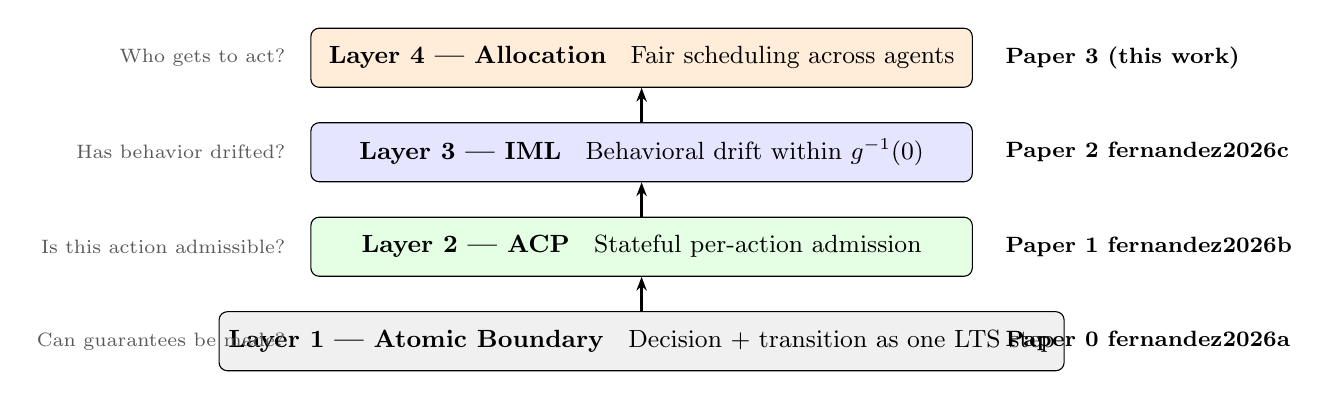
\begin{tikzpicture}[
  every node/.style={font=\small},
  box/.style={draw, rounded corners=3pt, minimum width=8.4cm,
              minimum height=0.75cm, align=center},
  lbl/.style={font=\footnotesize\bfseries, anchor=west},
  qst/.style={font=\scriptsize, anchor=east, text=gray!70!black},
  arr/.style={-{Stealth[length=5pt]}, thick},
  >=Stealth
]

% ── Layer 4 (top) ─────────────────────────────────────────────
\node[box, fill=orange!15]  (L4) at (0, 3.6)
  {\textbf{Layer 4 — Allocation} \;
   {\normalfont Fair scheduling across agents}};

% ── Layer 3 ───────────────────────────────────────────────────
\node[box, fill=blue!10] (L3) at (0, 2.4)
  {\textbf{Layer 3 — IML} \;
   {\normalfont Behavioral drift within $g^{-1}(0)$}};

% ── Layer 2 ───────────────────────────────────────────────────
\node[box, fill=green!10] (L2) at (0, 1.2)
  {\textbf{Layer 2 — ACP} \;
   {\normalfont Stateful per-action admission}};

% ── Layer 1 (bottom) ──────────────────────────────────────────
\node[box, fill=gray!12]  (L1) at (0, 0)
  {\textbf{Layer 1 — Atomic Boundary} \;
   {\normalfont Decision $+$ transition as one LTS step}};

% ── Arrows ────────────────────────────────────────────────────
\draw[arr] (L1.north) -- (L2.south);
\draw[arr] (L2.north) -- (L3.south);
\draw[arr] (L3.north) -- (L4.south);

% ── Right-hand labels ─────────────────────────────────────────
\node[lbl] at (4.5, 3.6)  {Paper~3 (this work)};
\node[lbl] at (4.5, 2.4)  {Paper~2 \citep{fernandez2026c}};
\node[lbl] at (4.5, 1.2)  {Paper~1 \citep{fernandez2026b}};
\node[lbl] at (4.5, 0)    {Paper~0 \citep{fernandez2026a}};

% ── Left-hand questions ───────────────────────────────────────
\node[qst] at (-4.4, 3.6) {Who gets to act?};
\node[qst] at (-4.4, 2.4) {Has behavior drifted?};
\node[qst] at (-4.4, 1.2) {Is this action admissible?};
\node[qst] at (-4.4, 0)   {Can guarantees be made?};

\end{tikzpicture}
\caption{The four-layer governance architecture.
  Each layer addresses a governance failure invisible to the layer below.
  Layer~1 (Paper~0): structural impossibility of split systems;
  establishes the atomic boundary as the minimal correctness requirement.
  Layer~2 (Paper~1, ACP): per-action admission control enforced atomically
  via Execution Tokens.
  Layer~3 (Paper~2, IML): detection of behavioral drift within the
  compliance region $g^{-1}(0)$ where enforcement is structurally blind.
  Layer~4 (this paper): fair scheduling of which agent presents its
  request to the atomic boundary, preventing Sybil amplification and
  allocation-level concentration.
  The layers are non-redundant: correctness at Layer~$k$ does not imply
  correctness at Layer~$k+1$.}
\label{fig:fourlayer}
\end{figure}

The non-redundancy claim deserves emphasis.  A system at Layer~1
satisfies the atomic boundary but may fail Layers~2--4.  A system
at Layer~2 (ACP) is atomically correct and enforces bounded
per-action admission, but (by Theorem~\ref{thm:necessity}) may fail
Layers~3--4.  A system at Layer~3 (IML-equipped) monitors behavioral
drift but does not address which agent gets access to the boundary
(Layer~4).  Only a system operating at all four layers simultaneously
provides the full governance guarantee: no inadmissible action fires
(Layers~1--2), behavioral drift from admission-time contracts is
detected (Layer~3), and admissible actions are distributed fairly
across agents and actors (Layer~4).

Crucially, each layer \emph{assumes} the layer below it is functioning:
IML takes atomicity as given; the allocation layer takes ACP enforcement
as given.  This layered dependency is not circular but
\emph{compositional}: each paper in the series contributes a component
that is necessary but not sufficient alone, and the quartet is closed
exactly when all four components are present.

% ============================================================
\section{Discussion and Related Work}
\label{sec:discussion}
% ============================================================

%  ── Content outline ───────────────────────────────────────────────────────
%
%  8.1 Relationship to classical fairness theory
%      - Max-min fairness (Demers et al., 1989; Bertsekas & Gallager)
%      - Proportional fairness (Kelly et al., 1998)
%      - Envy-freeness (Foley 1967; Varian 1974)
%      - Gibbard-Satterthwaite: our strategy-proofness impossibility is
%        a governance-layer analogue of the G-S theorem for resource
%        allocation under bounded enforcement
%
%  8.2 Relationship to Sybil attack literature
%      - Douceur 2002: original Sybil attack in P2P
%      - Cheng & Friedman 2005: Sybil-proofness in reputation systems
%      - Our contribution: formal Sybil characterization in the LTS/ACP model
%
%  8.3 Relationship to multi-agent resource allocation
%      - Chevaleyre et al. 2006: fair division of indivisible goods
%      - Bouveret & Lemaître 2016: fairness in combinatorial domains
%      - Our model is continuous (shares of a divisible capacity K)
%      - The atomicity constraint makes it a scheduling problem, not
%        a static allocation problem
%
%  8.4 Relationship to the governance quartet
%      - Paper 0: structural necessity of atomic boundaries
%      - Paper 1: ACP instantiation — shows M1 is correct but not fair
%      - Paper 2: IML operates above the boundary and complements M3/M4
%      - This paper: closes the quartet — what must be fair at the
%        scheduling layer above the decision boundary
%
%  8.5 Limitations
%      - We assume a fixed population N; dynamic joins/leaves not modeled
%      - Actor mapping π assumed stable; churn creates identification challenges
%      - We study worst-case fairness; average-case analysis under stochastic
%        arrivals is left to future work
%      - Interaction with ACP's BAR-Monitor: not yet characterized
%
%  ─────────────────────────────────────────────────────────────────────────

\subsection{Relationship to Classical Fairness Theory}
\label{sec:related-fair}

Fair resource allocation has a long history in both economics and
networking.  \emph{Max-min fairness}~\citep{demers89, bertsekas87}
maximizes the minimum share across all agents, naturally preventing
starvation.  \emph{Proportional fairness}~\citep{kelly98} maximizes
the sum of logarithmic utilities, distributing capacity proportionally
to demand.  \emph{Envy-freeness}~\citep{foley67, varian74} requires
that no agent prefers another's allocation.

Our work departs from classical fair-division theory in three respects.
First, the resource being allocated is not a divisible good but
\emph{access to an indivisible atomic boundary}: each ``quantum'' of
capacity is one evaluation step of $F$, and the boundary can only
process one request at a time.  Second, the correctness constraint
(each admitted action must be admissible) interacts with the fairness
constraint: we cannot simply round-robin all agents regardless of
their admissibility state.  Third, the actor structure
(Definition~\ref{def:actors}) introduces an identity layer absent
from classical models, giving rise to the Sybil amplification problem.

The strategy-proofness impossibility (Theorem~\ref{thm:strategy}) is a
governance-layer analogue of the Gibbard--Satterthwaite
theorem~\citep{gibbard73, satterthwaite75}: just as no voting rule can
be simultaneously non-dictatorial, Pareto-efficient, and
strategy-proof, no per-agent-independent allocation mechanism can
simultaneously guarantee actor-level proportionality and
strategy-proofness against identity fragmentation.

\subsection{Relationship to the Sybil Attack Literature}
\label{sec:related-sybil}

The Sybil attack was formally identified by \citet{douceur02} in the
context of peer-to-peer reputation systems: a malicious node creates
multiple fake identities to subvert voting or reputation aggregation.
Identity-based defenses (trusted authorities, admission fees, resource
costs) are the standard mitigations.

Our contribution is distinct: we provide a formal characterization of
Sybil amplification within the LTS-based governance model, prove that
it is consistent with full atomic correctness, and show that the
mitigation (M3, actor-aware allocation) requires actor-state
aggregation that trades off per-agent independence.  Crucially, in our
setting the ``Sybil nodes'' are not fake: they are legitimate agents
operating within their individual bounds.  The attack surface is not
dishonesty but the structural separation between per-agent enforcement
and system-wide allocation.

\subsection{Relationship to Multi-Agent Resource Allocation}
\label{sec:related-marl}

The formal study of multi-agent resource allocation~\citep{chevaleyre06}
concerns the distribution of indivisible goods among self-interested
agents, asking which allocations are efficient, envy-free, or
Pareto-optimal.  Our setting shares several features---multiple agents,
limited capacity, competing interests---but departs in three important
ways.

First, the \emph{resource} in our model is not a good but an
\emph{access right to a governance mechanism}.  The atomic boundary $F$
is the resource being allocated; execution capacity is its product.
Unlike goods, access rights have a correctness dimension: the allocation
mechanism must respect the admissibility predicate $\Adm$, which can
refuse a request regardless of allocation priority.  Fair-division theory
does not include this constraint.

Second, our model is \emph{sequential}: the allocation unfolds over time
as agents submit requests and the LTS evolves.  Fair-division results
typically concern static one-shot assignments.  The temporal failure
modes we identify---temporal domination, starvation---are inherently
dynamic and have no counterpart in static allocation theory.

Third, the actor-agent structure introduces a \emph{strategic layer}
absent from standard models: actors can manipulate their effective
share by adjusting the number of agents they control, which is not a
strategic variable in fair-division models where agents are primitive.
The Gibbard--Satterthwaite analogue we prove (Theorem~\ref{thm:strategy})
addresses this strategic dimension and has no standard fair-division
counterpart.

These three departures---correctness constraints, temporal dynamics, and
strategic identity control---define the specific contribution of the
present work relative to fair-division theory.

\subsection{Position within the Governance Quartet}
\label{sec:related-quartet}

The four papers in this series form a logically closed architecture;
Table~\ref{tab:quartet} summarizes each paper's question, result, and
the failure mode it addresses.

\begin{table}[h]
\centering
\caption{The governance quartet: question, result, and failure mode addressed.}
\label{tab:quartet}
\small
\begin{tabular}{lp{3.2cm}p{3.6cm}p{3.0cm}}
\toprule
\textbf{Paper} & \textbf{Question} & \textbf{Central result} &
  \textbf{Failure mode} \\
\midrule
0 \citep{fernandez2026a}
  & When can admissibility be guaranteed?
  & Split systems cannot guarantee it; atomicity is necessary and sufficient.
  & TOCTOU / state change between decision and execution \\[4pt]
1 \citep{fernandez2026b}
  & How to implement the atomic boundary?
  & ACP: Execution Token issued and consumed atomically with ledger mutation.
  & Per-action correctness under concurrent agents \\[4pt]
2 \citep{fernandez2026c}
  & Does correct enforcement imply behavioral alignment?
  & No: $\mathcal{A}_0 \notin \sigma(g)$; IML restores observability.
  & Behavioral drift invisible to enforcement \\[4pt]
3 (this work)
  & Does correct admission imply fair allocation?
  & No: Theorems~\ref{thm:sybil}--\ref{thm:strategy}; allocation layer is necessary.
  & Sybil amplification and cross-agent distribution failure \\
\bottomrule
\end{tabular}
\end{table}

The papers are \emph{non-redundant} in the sense that the result of each
is invisible to the prior layers: admissibility failures in split systems
(Paper~0) cannot be detected by policy engines that are split by
construction; behavioral drift (Paper~2) cannot be detected by
enforcement signals; allocation skew (this paper) cannot be detected
by the IML, which monitors individual agents in isolation.  Together,
they cover the full governance space from execution-time correctness to
system-wide distributional fairness.

\subsection{Limitations and Future Work}
\label{sec:limitations}

Two important questions are left for future work.  First, we assume
a fixed agent population; dynamic arrival and departure of agents
introduces challenges for actor-aware mechanisms (how to reallocate
$K_U$ when actors join or leave) that are outside the scope of the
present LTS model.  Second, we analyze worst-case fairness; a
stochastic model of request arrivals would permit average-case
analysis and tighter bounds on the detection-delay amplification of
Corollary~\ref{cor:underservice}.

The two questions previously listed as open---the interaction between
M3 and ACP's BAR-Monitor, and the formal treatment of misrepresented
actor mappings---have been resolved in
\S\ref{sec:bar-interference} (Proposition~\ref{prop:bar-m3} and
Remark~\ref{rem:bar-correction}) and in the M3 analysis
(Proposition~\ref{prop:pi-misrep} and Remark~\ref{rem:pi-obs}),
respectively.

% ============================================================
\section{Conclusion}
\label{sec:conclusion}
% ============================================================

%  ── Content outline ───────────────────────────────────────────────────────
%
%  Paragraph 1: Restate the core result
%  "Atomic correctness is a necessary but not sufficient condition for
%   governance.  A system that is atomically correct at every decision point
%   can still fail arbitrarily at the allocation layer."
%
%  Paragraph 2: The three theorems in plain language
%  - Sybil: per-agent enforcement linearly amplifies actor capacity
%  - Necessity: fairness requires an explicit allocation layer
%  - Strategy-proofness: you can't have independence + proportionality + SP
%
%  Paragraph 3: The four mechanisms and the tradeoff
%  M1/M2 are simple but Sybil-vulnerable.
%  M3/M4 achieve fairness at the cost of actor-state aggregation.
%  The right choice depends on whether π is observable.
%
%  Paragraph 4: The quartet closure
%  Paper 0: what is admissible (structural)
%  Paper 1: how admissibility is enforced (protocol)
%  Paper 2: how behavioral drift is measured (monitoring)
%  Paper 3: how admissible actions are distributed (fairness)
%  "Together, these four layers constitute a complete governance
%   architecture for autonomous agent systems."
%
%  Closing sentence: "Correctness is local. Fairness is global. Both
%   are necessary for governed autonomy."
%
%  ─────────────────────────────────────────────────────────────────────────

We have introduced the \emph{allocation layer} as a necessary addition
to atomic governance architectures.  Using the LTS framework of
\citet{fernandez2026a}, we proved that a system can be atomically
correct at every admission decision while simultaneously failing at the
distribution of those decisions across agents.  Correctness is a local
property of state transitions; fairness is a global property of
scheduling patterns.  Neither implies the other.

The Sybil Amplification Theorem establishes the precise mechanism of
failure: per-agent bounded enforcement scales linearly with agent count,
enabling an actor to multiply its governance capacity without bound by
registering additional agents.  The Allocation Necessity Theorem
establishes that no property of the atomic boundary function $F$ can
prevent this---a separate allocation mechanism above the boundary is
required.  The Strategy-Proofness Impossibility establishes the
fundamental tradeoff: per-agent independence, actor-level
proportionality, and resistance to identity fragmentation cannot all be
achieved simultaneously.

The four allocation mechanisms we analyze navigate this tradeoff from
different positions.  Simple mechanisms (M1, M2) preserve per-agent
independence but are Sybil-vulnerable.  Actor-aware mechanisms (M3,
M4 with actor weights) achieve proportionality and strategy-proofness
but require cross-agent state aggregation and observability of the
actor mapping.  Deployers of multi-agent governance infrastructure
must choose based on whether $\owner$ is observable and whether
identity fragmentation is a realistic threat in their environment.

This paper closes the governance quartet.  Paper~0~\citep{fernandez2026a}
establishes that admissibility can only be guaranteed by atomic
enforcement: the decision boundary is a structural necessity, not an
engineering choice.  Paper~1~\citep{fernandez2026b} instantiates the
boundary as ACP and demonstrates its correctness properties across
thousands of states.  Paper~2~\citep{fernandez2026c} shows that
enforcement-correct behavior can still drift from admission-time
contracts, and introduces IML to detect this drift.  The present paper
shows that a drift-monitored, atomically correct system can still
allocate its governance capacity unfairly---and provides the formal
tools to characterize, prevent, and detect this failure.

\begin{quote}
\textit{Admission control determines what can happen.
Fairness determines who gets to act.
Correctness is local. Fairness is global.
Both are necessary for governed autonomy.}
\end{quote}

% ============================================================
% Bibliography
% ============================================================
\bibliographystyle{plainnat}
\bibliography{references}

\end{document}
